\chapter{Performances of the Different Numerical Methods}
\label{chapterPerformances}
As seen in chapter~\ref{chapter_caseStudy}, the privileged numerical technique we employed to study our model is the MPO method. However, other two methods have been analyzed and implemented for the same purpose, but with different performances: the QT method has been useful only for size chain of 8 and 10 sites, i.e. it has been useful in order to compare the MPO results and to confirm their plausibility, while CSR method has revealed not to be a suitable method for the study of this kind of models. In the present chapter, we show the limitations of CSR method for the case of 4-sites chain (for which we can perform a direct numerical integration of the master equation) and in the following sections, a comparison between QT and MPO results and a brief analysis of their convergence and numerical errors are shown.

\section{The CSR Method: Limitations and Usability}
The CSR method, described in section~\ref{chapter3_csr}, has been studied and implemented in order to analyze the model described in the last chapter. The algorithm is written in pseudocode in appendix~\ref{AppendixA}.

In this section, we show that the CSR method is not a fitting method for investigating systems described by a model such as the one under consideration.

In order to prove this, we can see the case of a 4-sites chain for the proposed model. In particular, we can study the magnetization profile along z direction, i.e. the steady-state expectation value $\langle \sigma_i^z \rangle$ of the Pauli spin- matrix $\sigma^z$ for each site:
\begin{equation*}
    \langle \sigma_i^z \rangle = \Tr(\sigma_i^z \rho_S),
\end{equation*}
being $\rho_S$ the steady-state density matrix of the system.

The Hilbert space $\mathcal{H}$ corresponding to a chain made up by 4 spin-1/2 has dimension of $2^{4} = 16$, so the number of states that describe the system are $2^4$. If the method works, the system will be described by a number of states $M < \dim(\mathcal{H})$, i.e. $M < 16$, in the case under consideration.

In the upper panel of fig.~\ref{fig:4sites_LM_convergenceIncreasingM}, it is clear that for such a system the convergence has not been reached. Even for $M = 15$, with a number of states that cover almost the full Hilbert space, the results are not the convergent ones (shown in black). On the other hand, if we consider a model in which every site is coupled to a dissipator, we can see how the magnetization profile gets to convergence starting from $M = 9$ already, for almost all sites. 

\begin{figure}[H]
    \centering
    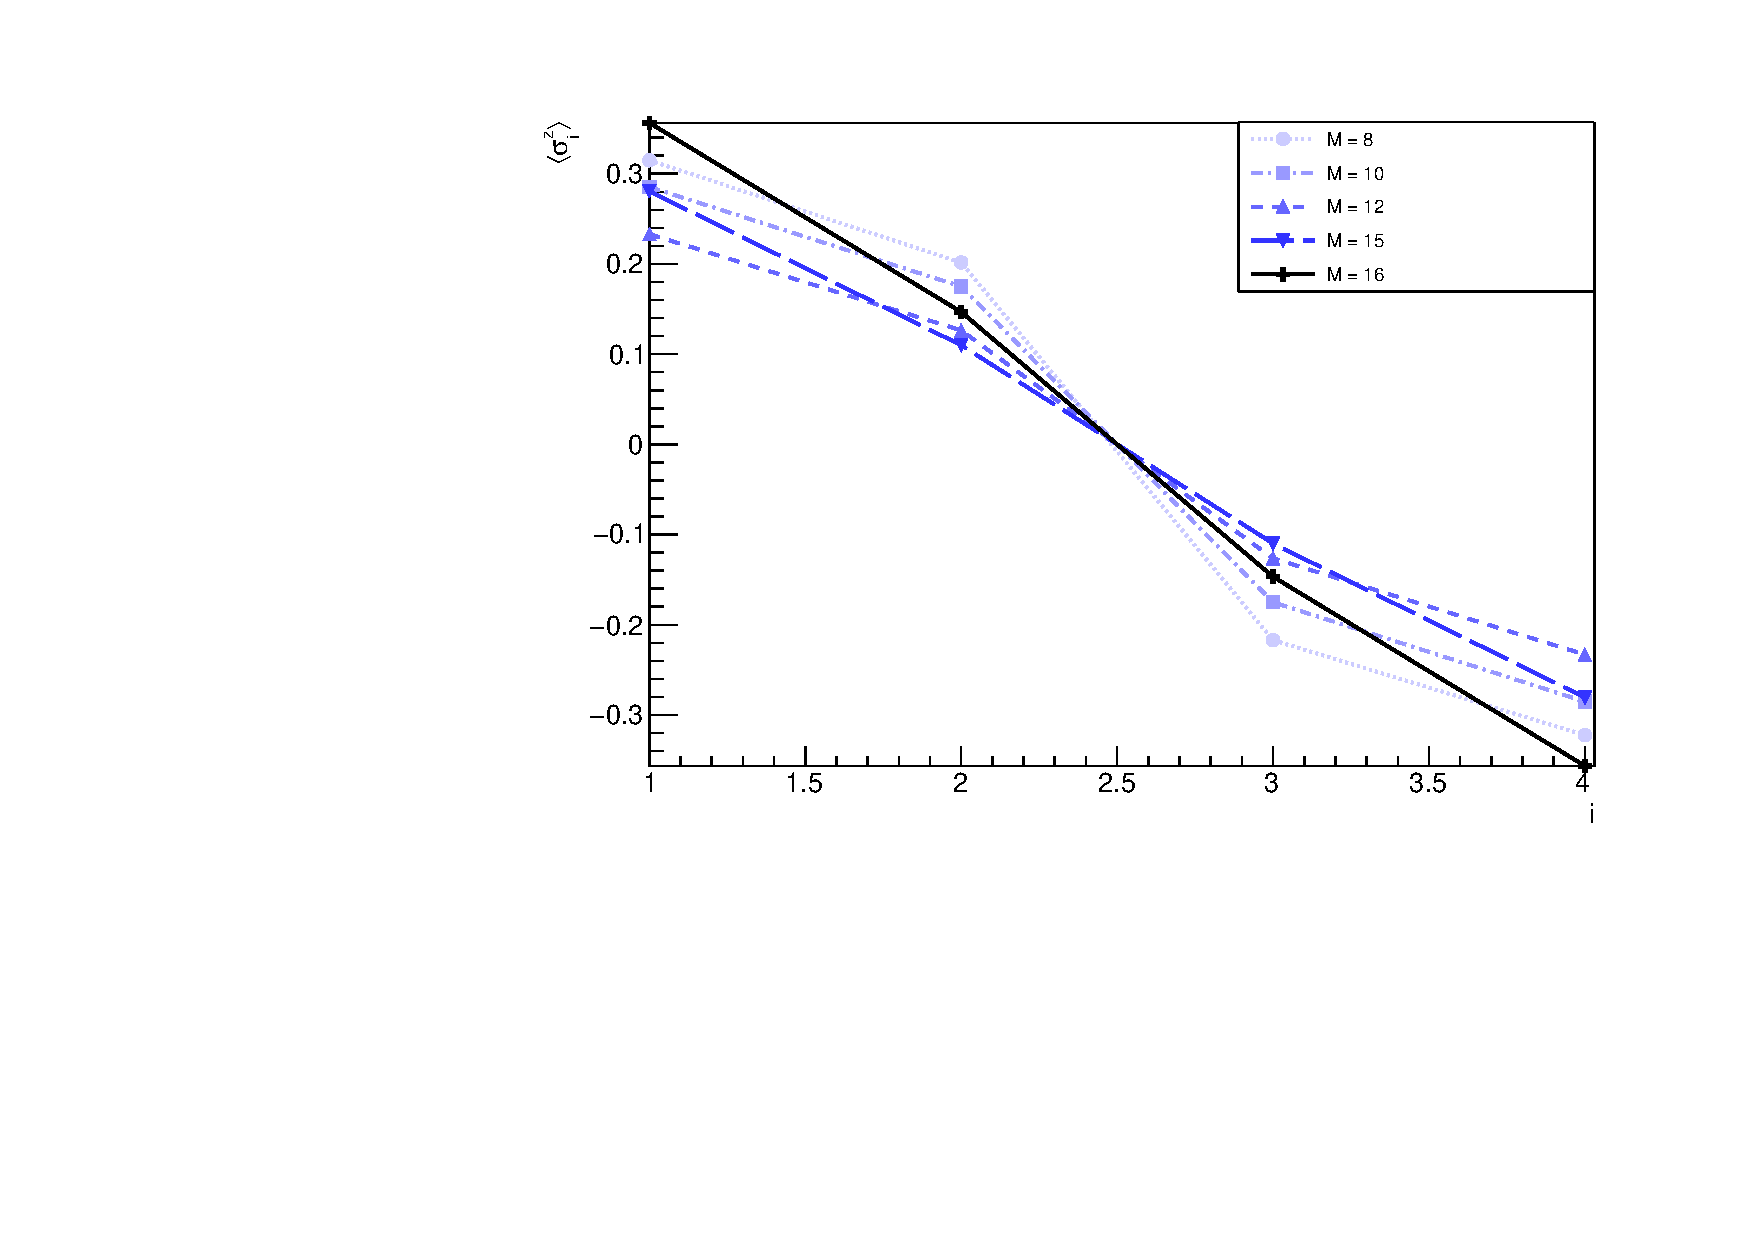
\includegraphics[scale=0.5]{Figures/4sites/4sites_LM_convergenceIncreasingM.pdf}
    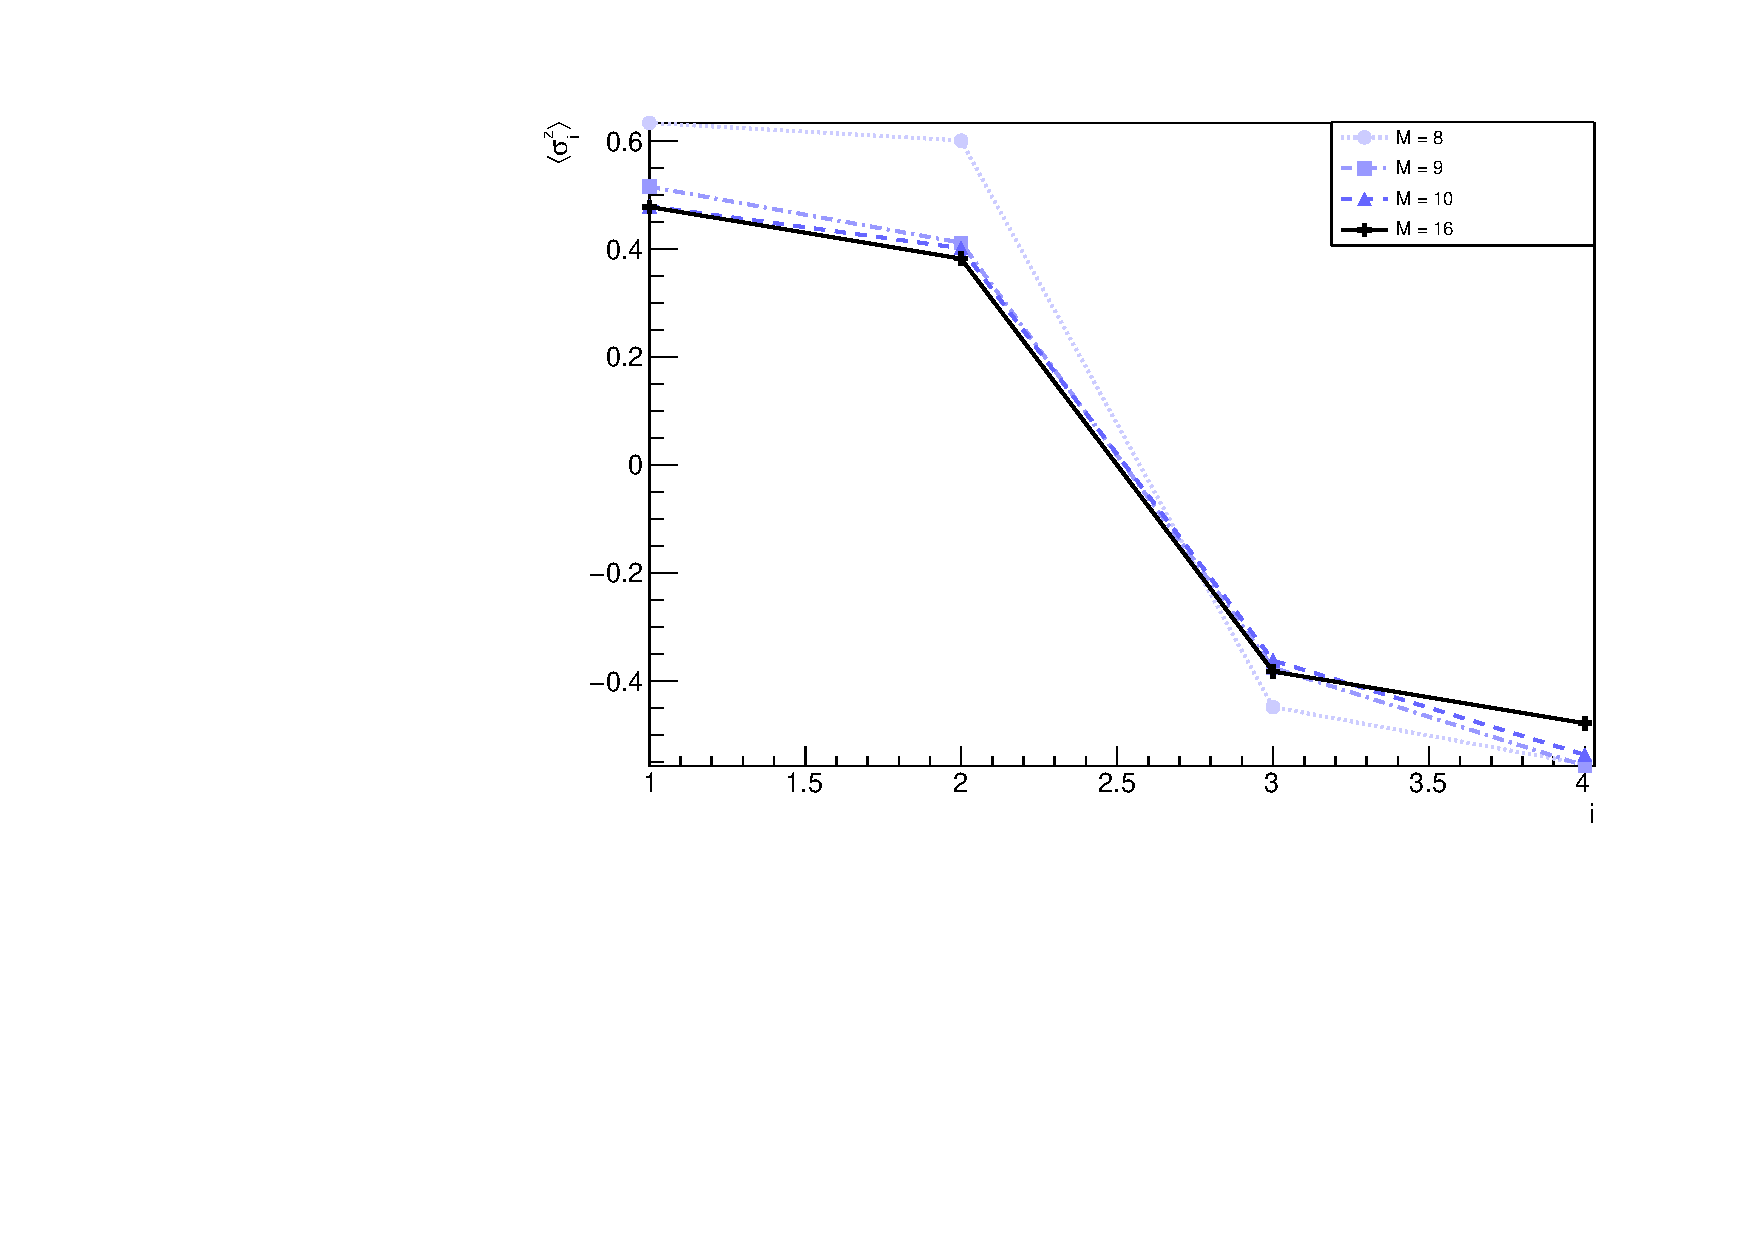
\includegraphics[scale=0.5]{Figures/4sites/4sites_totalDissipators.pdf}
    \captionsetup{width=1.\linewidth}
    \caption{Upper panel: spin profile of a 4-sites chain for the model described above with $J_z=1$ and $\gamma = 1 $ for several values of corner-space dimension $M$. The black markers and lines are those representing the expectation value of the magnetization calculated by means of a complete set of states of Hilbert space (which has dimension $2^4$).
    Bottom panel: spin profile of the same chain, but in this case every spin of the chain is coupled to a dissipator. Here, the convergence is (almost) reached for $M<\text{dim}(\mathcal{H})$.}
    \label{fig:4sites_LM_convergenceIncreasingM}
\end{figure}

In order to confirm the limitations of this method, the same comparison is done for a longer chain, made up by 8 sites. In this case, the results of CSR method are compared to those of MPO method, since a brute-force diagonalization of the Liouvillian operator would not be possible: it would require a huge amount of memory. As already mentioned previously, the MPO method results are proved to be plausible. In the two panels of fig.~\ref{fig:comparisonCSR_MPO_8site}, it is clear that the convergence has not been reached in none of the cases, but in the second one (the bottom panel) the profile is slightly more similar to the one obtained from MPO method. Moreover, in both cases there is no significant difference between the results obtained for $M = 50$ and $M = 100$ (upper panel of fig.~\ref{fig:comparisonCSR_MPO_8site}) and for $M = 50$ and $M = 80$ (bottom panel of fig.~\ref{fig:comparisonCSR_MPO_8site}). It is worth noting that the full Hilbert space for a 8-sites chain has dimension $2^{8} = 256$.

\begin{figure}[H]
    \centering
    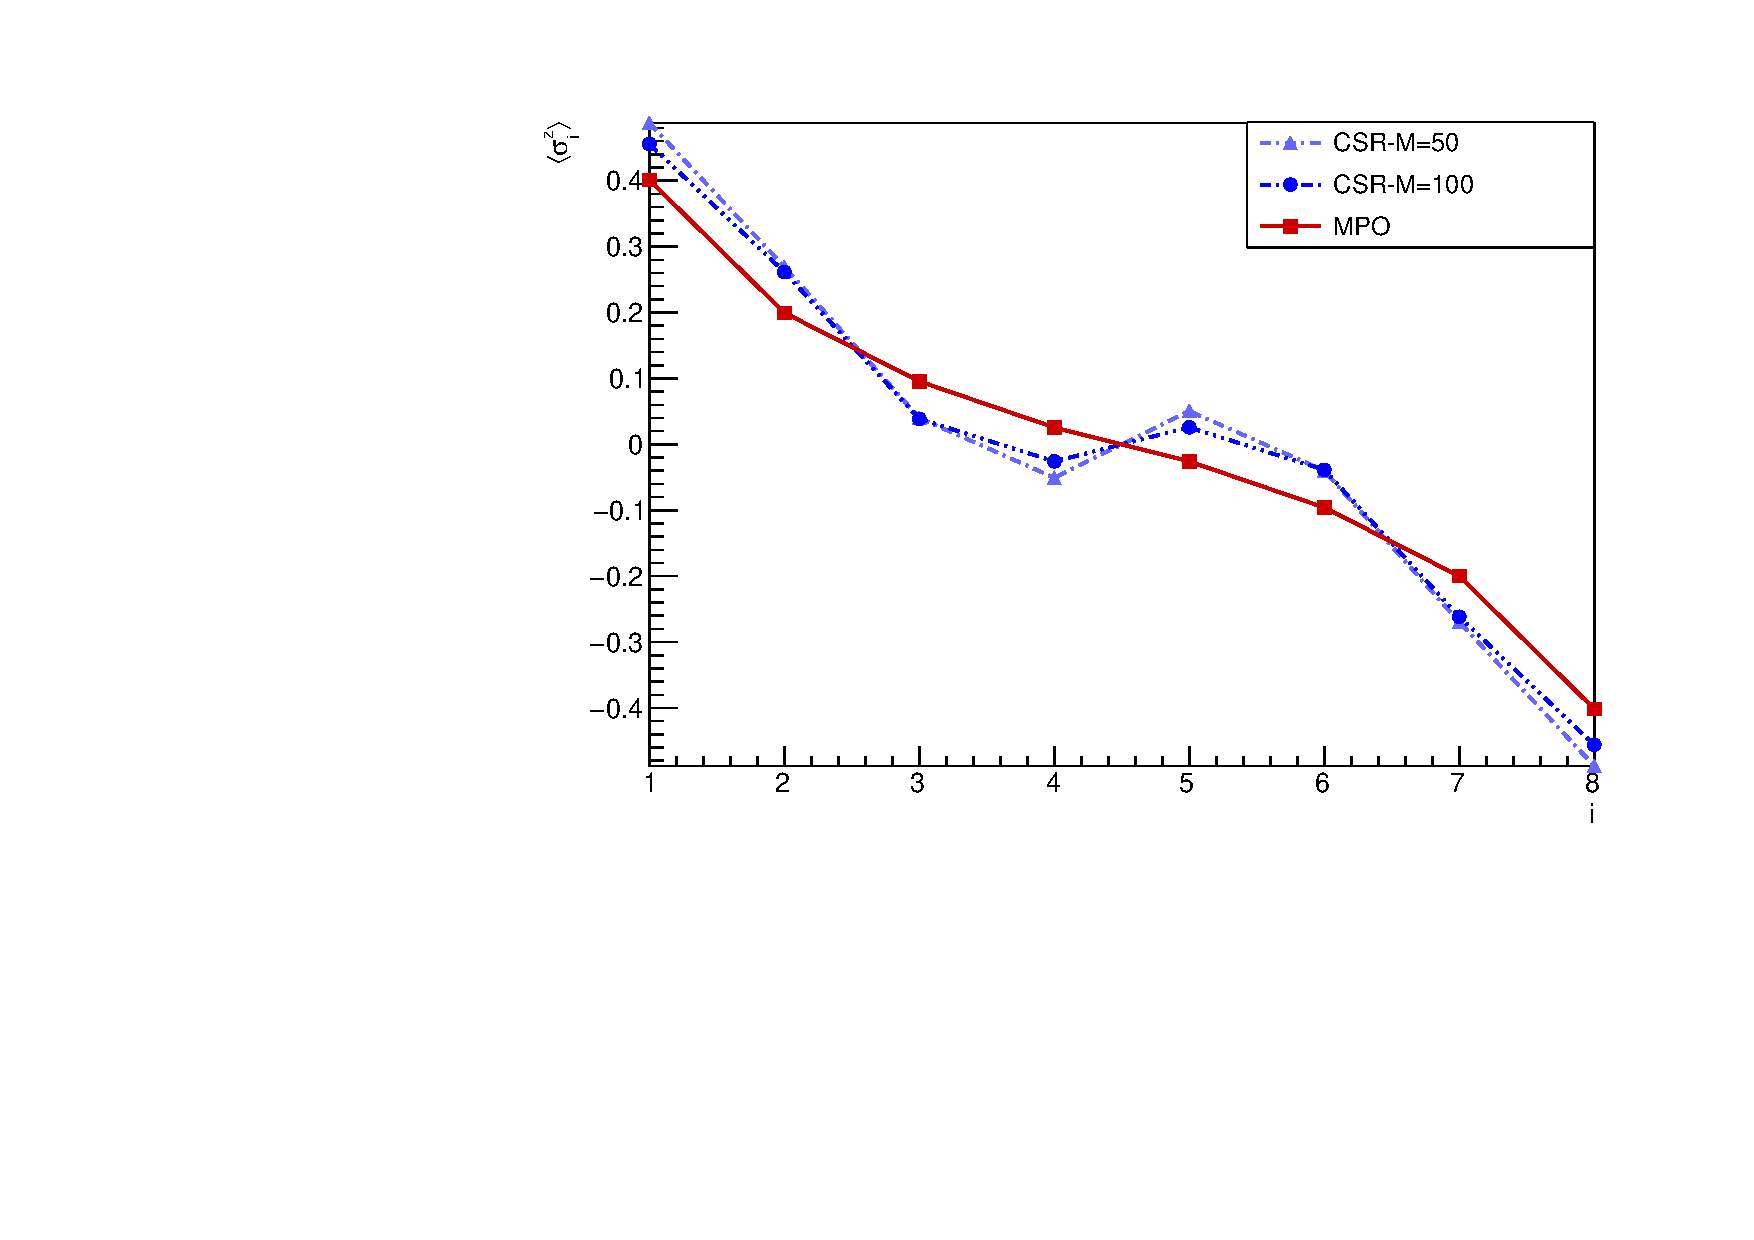
\includegraphics[scale=0.45]{Figures/8sites/1U1D_comparisonCSR_MPO_8site.pdf}
    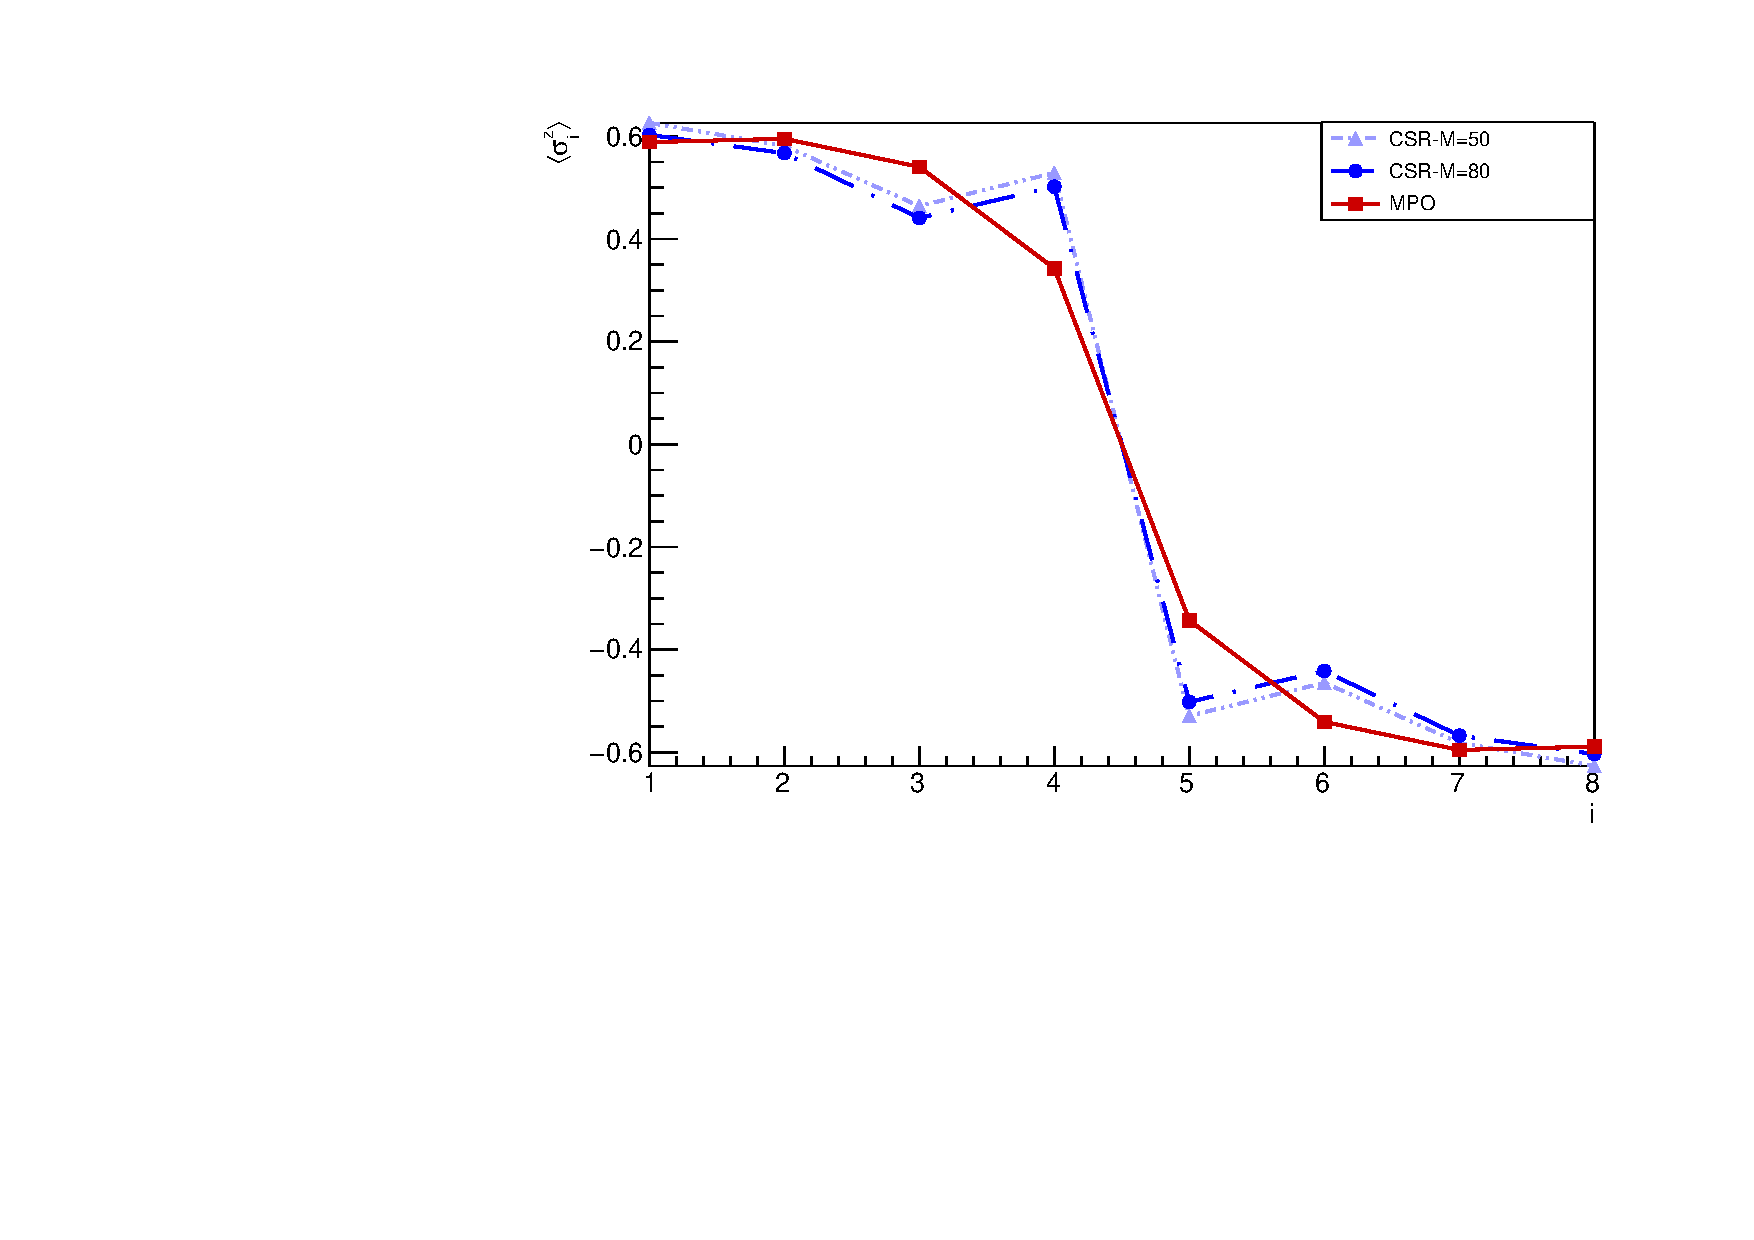
\includegraphics[scale=0.45]{Figures/8sites/8sites_MPOvsCORNER_4U4D.pdf}
    \captionsetup{width=1.\linewidth}
    \caption{Upper panel: spin profile of a 8-sites chain for the model described in sec.\ref{sec:model}. Bottom panel: spin profile of a 8-sites chain in which every spin of the chain is coupled to a dissipator. Data in red are obtained from MPO method, with m = 100 and T = 1000 and data in blue are obtained from CSR method.}
    \label{fig:comparisonCSR_MPO_8site}
\end{figure}

Fig.~\ref{fig:LMComparison16s1051} displays the magnetization profile along z direction of a 16-sites chain obtained by CSR and MPO methods. The full Hilbert space of such a chain has dimension $2^{16} = 65536$, while in the simulations using the CSR method, we have kept $M = 65$ states. One could think that the dimension of the corner-space is too little to reach the convergence, but in~\cite{PhysRevLett.115.080604}, the convergence is reached for corner-spaces with a smaller rate $\frac{M}{\dim(\mathcal{H})}$. In conclusion, the results obtained let us think that this is not a suitable numerical method for studying the kind of systems that we have the purpose to analyze in the present work.

\begin{figure}[H]
    \centering
    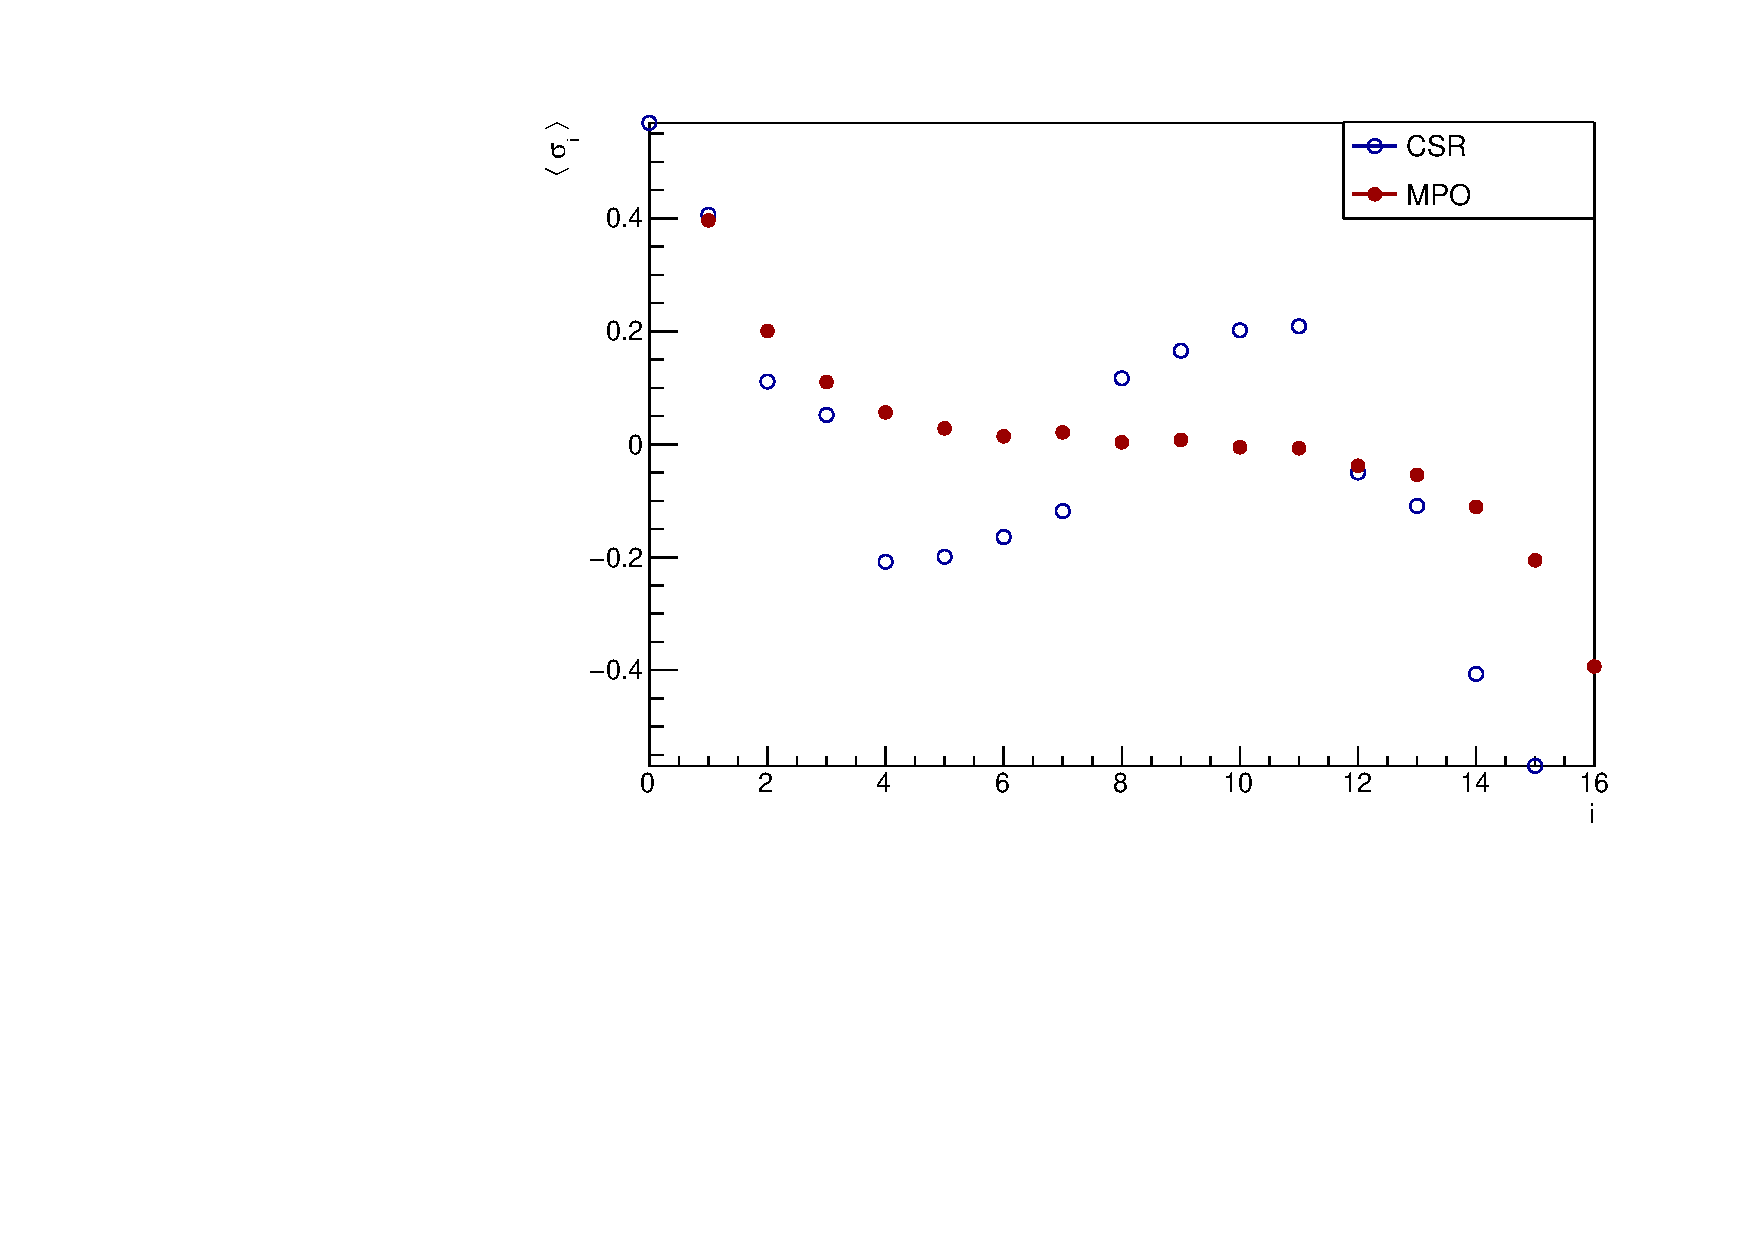
\includegraphics[scale=0.5]{Figures/16sites/LMComparison16s1051.pdf}
    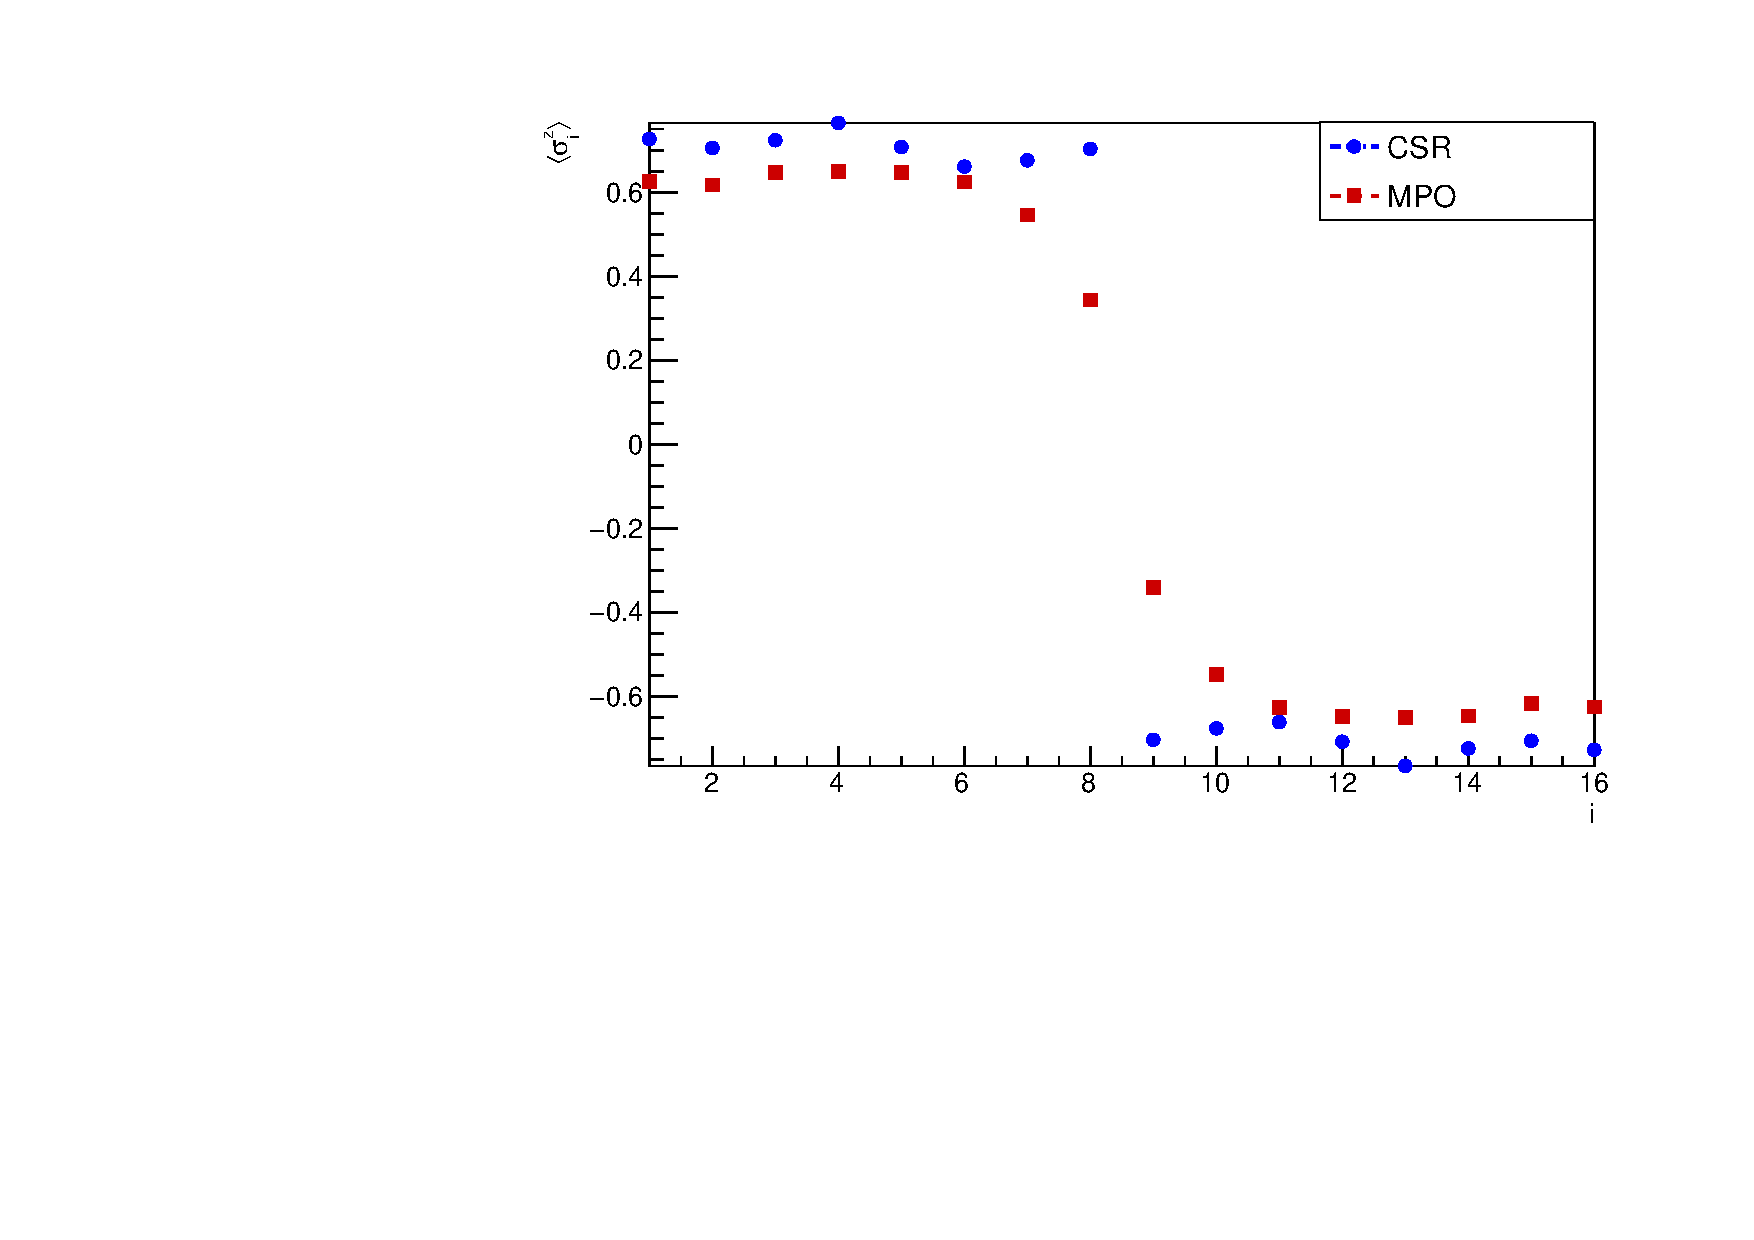
\includegraphics[scale=0.5]{Figures/8U8D_comparisonCSRvsMPO.pdf}
    \captionsetup{width=1.\linewidth}
    \caption{Upper panel: spin profile for a 16-sites chain for the model described in section~\ref{sec:model}. Bottom panel: spin profile for a 16-sites chain in which every spin of the chain is coupled to a dissipator. Data in red are obtained from MPO method, with m = 80 and T = 2000 and data in blue are obtained from CSR method, with M = 65. It is self-evident the inadequacy of the corner-space method, for the model under study. The dimension of the corner-space is $M=65$.}
    \label{fig:LMComparison16s1051}
\end{figure}

%%%%%%%%%%%%%%%%%%%%%%%%%%%%%%%%%%%%%%%%%%%%%%%%%%%%%%%%%%%%%%%
%%%%%%%%%%%%%%%%%%%%%%%%%%%%%%%%%%%%%%%%%%%%%%%%%%%%%%%%%%%%%%%
%%%%%%%%%%%%%%%%%%%%%%%%%%%%%%%%%%%%%%%%%%%%%%%%%%%%%%%%%%%%%%%
\section{Performance of the QT Method}
In this section we briefly discuss the convergence of the data and error calculus for the quantum trajectories method.

The QT method, explained in section~\ref{chapt3_qtm}, doing the stochastic unraveling of the master equation, builds the quantum trajectories after which it is named.  Every quantum trajectory corresponds to a simulated experiment and for the model under consideration, it has an oscillatory profile as that displayed in fig.~\ref{fig:QTrajectories3}. In order to stabilize the solution, for every quantum trajectory, the average in time is considered, starting from the end of the transient, which is needed for a solution of the Lindblad equation to converge towards the steady-state.

\begin{figure}[H]
    \centering
    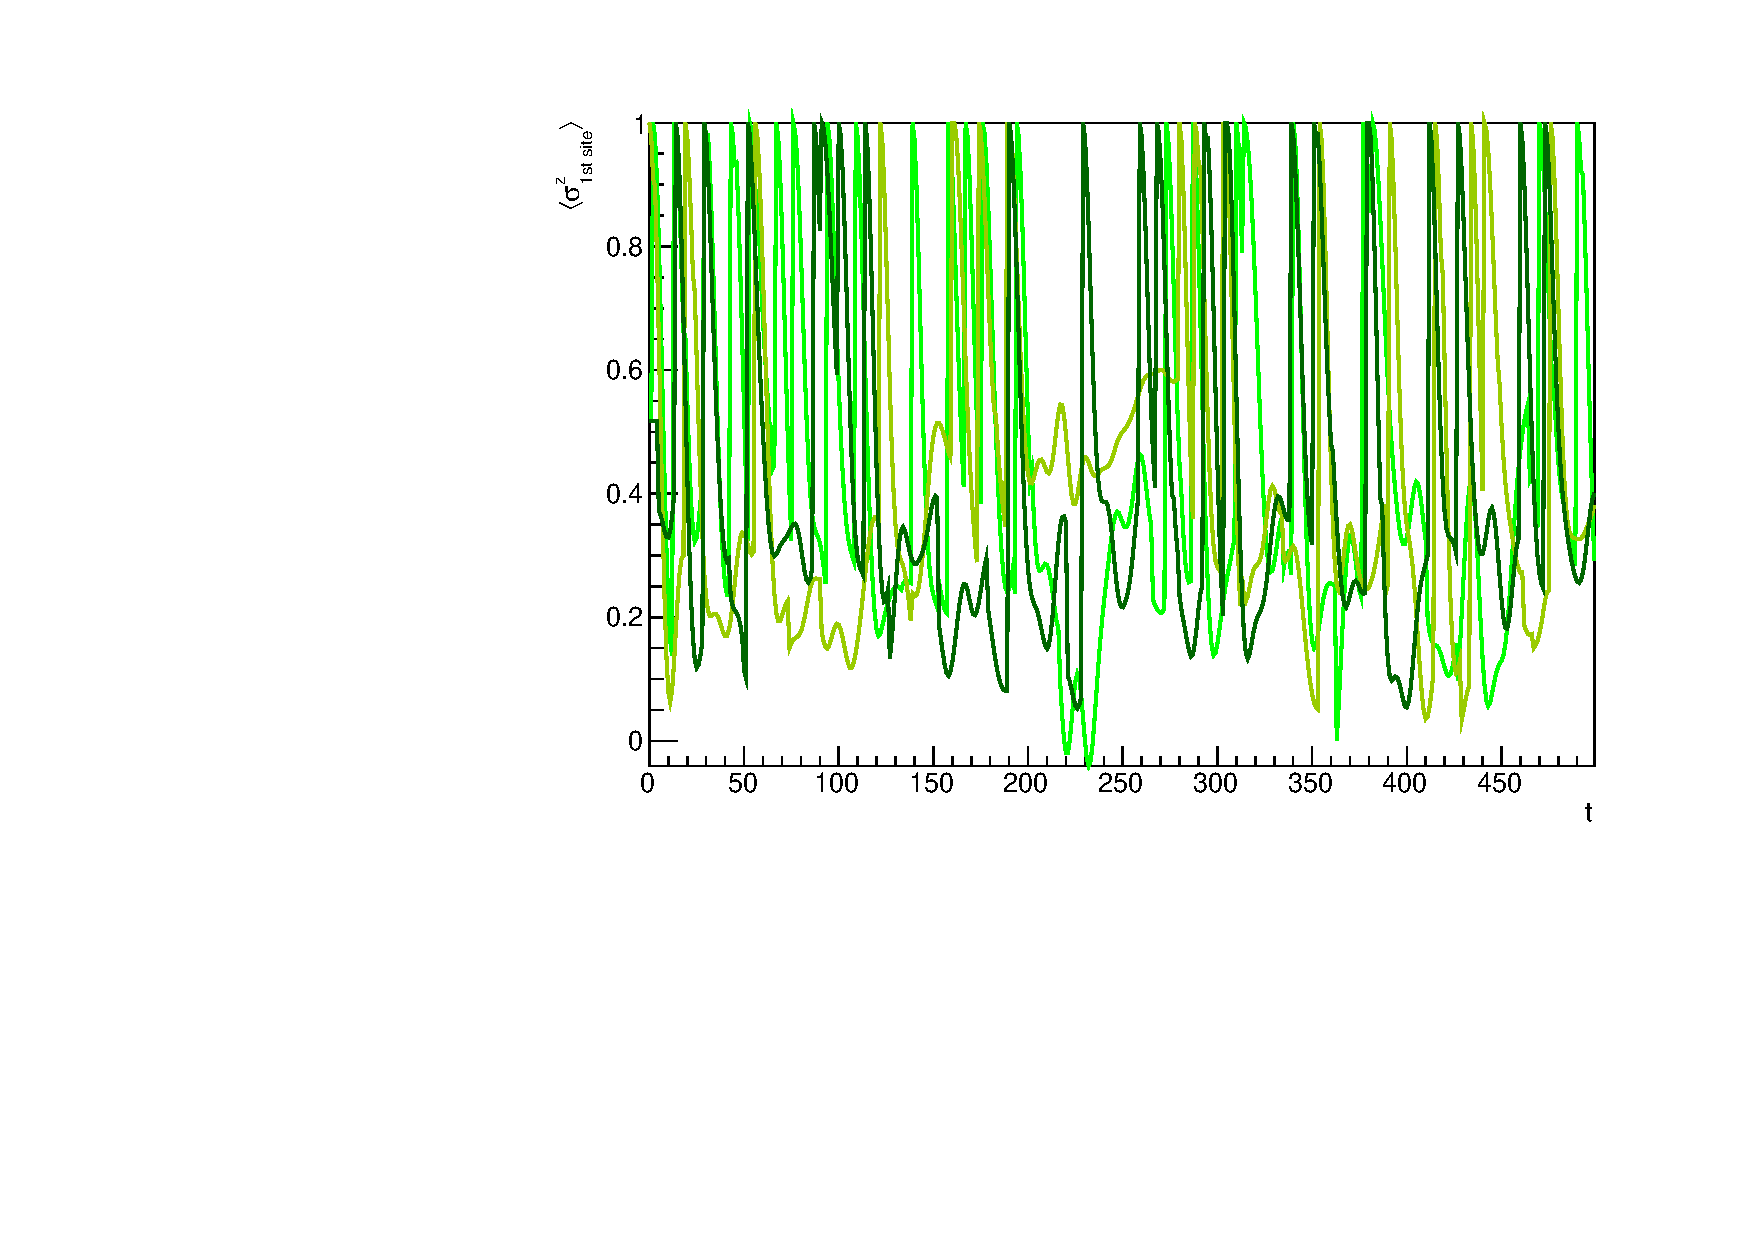
\includegraphics[scale=0.6]{Figures/QTrajectories3.pdf}
    \captionsetup{width=1.\linewidth}
    \caption{Example of three quantum trajectories displayed in different shades of green; in particular, this is the expectation value of the magnetization of the first site of the chain, for $J_z = 1$ and $\gamma = 1$. The total elapsed time is $T=500$, while the time step $dt = 0.1$.}
    \label{fig:QTrajectories3}
\end{figure}

For the same case considered in fig.~\ref{fig:QTrajectories3}, the convergence of the mean values over the number of events $N$ is shown in fig.~\ref{fig:Convergence_s8J1051}. 

\begin{figure}[H]
    \centering
    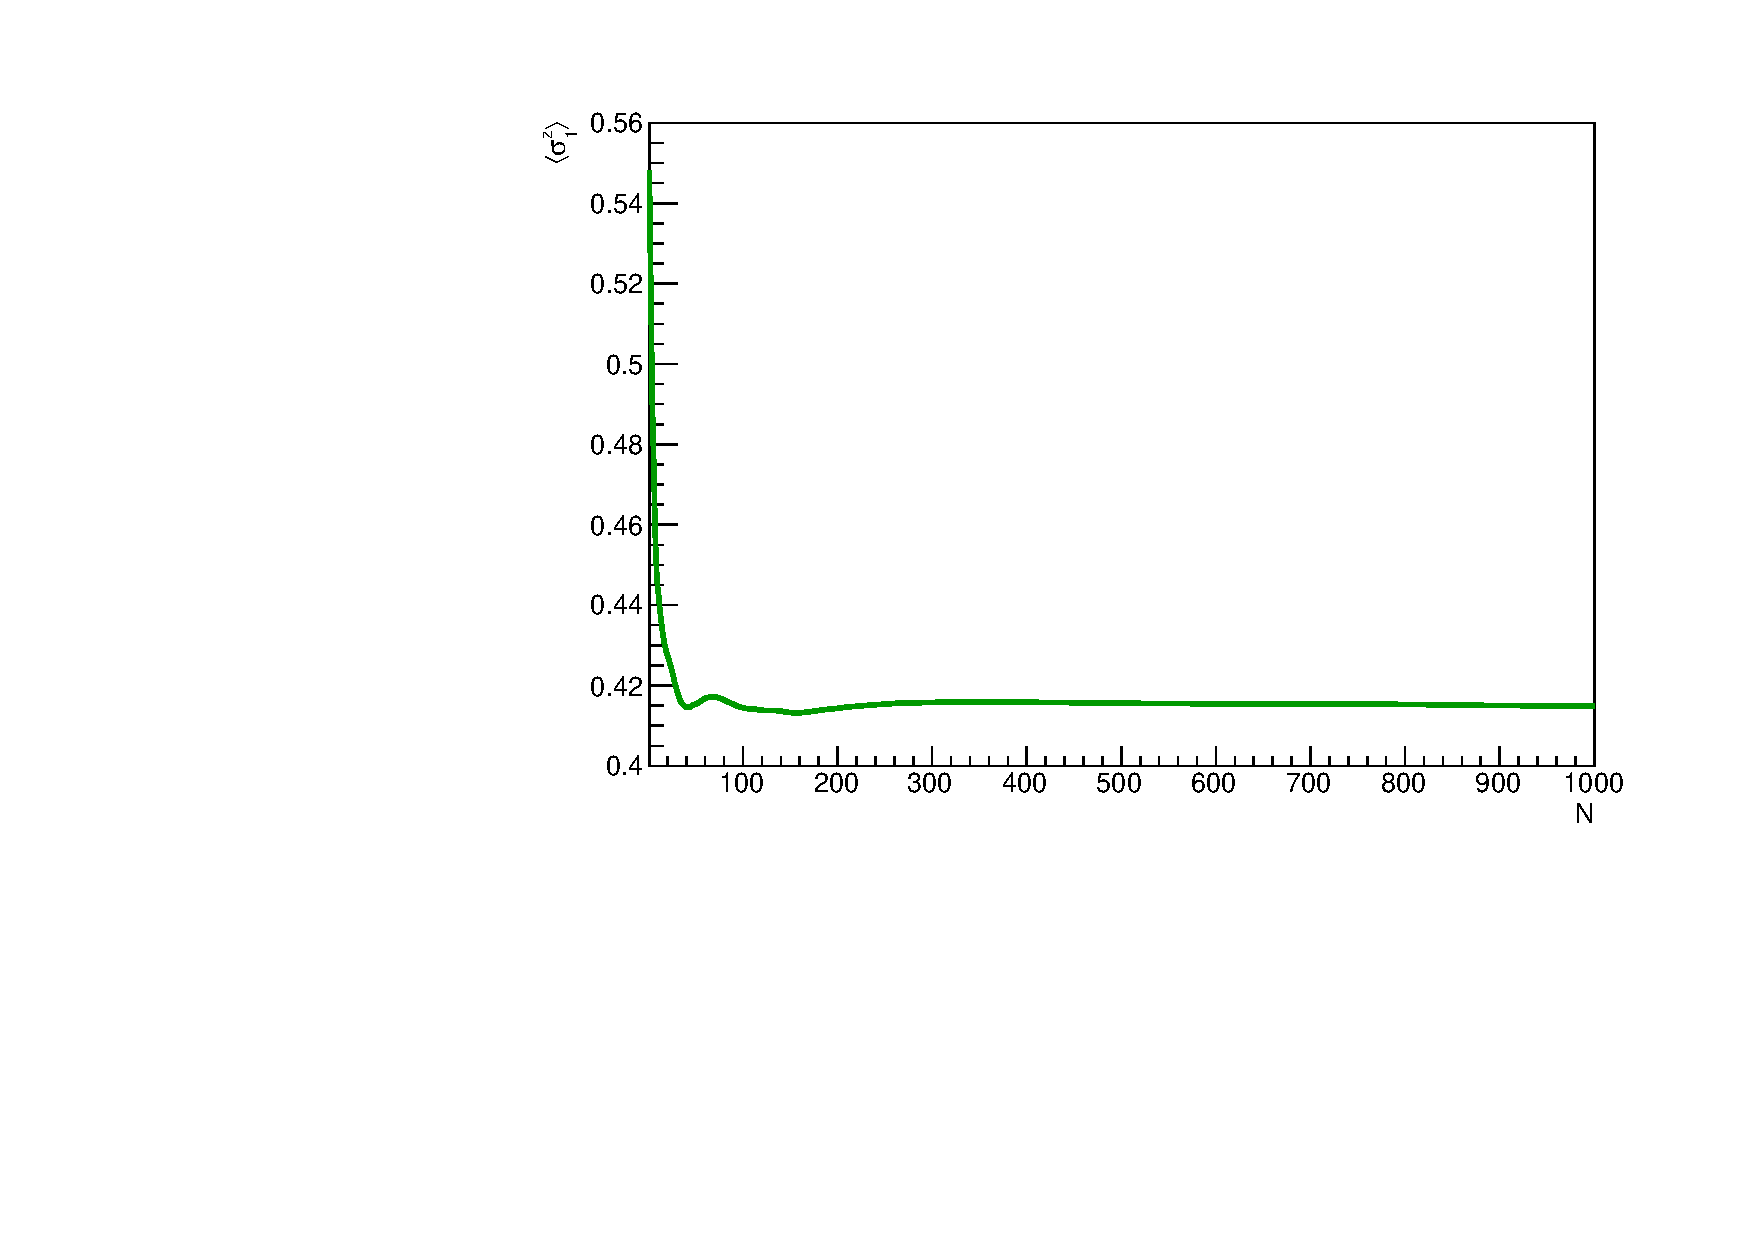
\includegraphics[scale=0.5]{Figures/Convergence_s8J1051.pdf}
    \captionsetup{width=1.\linewidth}
    \caption{Study of the convergence of the mean values of the quantum trajectories. For the case under consideration, the number of events is $N = 1000$.}
    \label{fig:Convergence_s8J1051}
\end{figure}

The study of the 8-sites chain was done with an elapsed time for every event of $T = 500$ and time-step $dt = 0.1$. The number of the simulated events is $N = 1000$.

The elapsed time for reaching the convergence with a characterization of the parameters as that explained above, is about $0.75$ hours. 

As numerical error, we have considered the standard deviation of the distribution of the mean.

%%%%%%%%%%%%%%%%%%%%%%%%%%%%%%%%%%%%%%%%%%%%%%%%%%%%%%%%%%%%%%%
%%%%%%%%%%%%%%%%%%%%%%%%%%%%%%%%%%%%%%%%%%%%%%%%%%%%%%%%%%%%%%%
%%%%%%%%%%%%%%%%%%%%%%%%%%%%%%%%%%%%%%%%%%%%%%%%%%%%%%%%%%%%%%%
\section{Performance of the MPO Method}
\label{sec:MPO_errors}
The convergence of MPO method depends essentially on the setting of two parameters: the bond dimension and the number of Trotter steps. The fig.~\ref{fig:convergence_8_12_16} shows the convergence profile of $\sigma^z$ for the first site of 8, 12, 16-sites chains for $J_z = 1$ and $\gamma = 1$. The same quantity can reach convergence in different times if, for example, $J_z$ assumes another value. 

In the present work, for 8-sites chains we considered a bond dimension $m = 100$ and Trotter steps in the range $[1200, 1500]$; for 12-sites chains we considered a bond dimension $m = 60$ and Trotter steps in the range $[1000, 2000]$; for 16-sites chains we considered a bond dimension $m = 80, 100, 140$ and Trotter steps in the range $[1000, 2500]$.

The elapsed time $t$ for reaching the convergence with these set of parameters, is the following:
\begin{itemize}
    \item $t \in [10', 20']$ for 8-sites chains;
    \item $t \in [30', 60']$ for 12-sites chains;
    \item $t \in [2 \text{ hours}, 4 \text{ hours}]$ for 16-sites chains.
\end{itemize}

The errors considered for the MPO method are merely the differences between two set of data obtained for two different bond dimensions. In particular, the error for an observable $O$, is given by:
\begin{equation*}
    \epsilon = |\braket{O}_{m_>} - \braket{O}_{m_<}|,
\end{equation*}
where $m_>$ ($m_<$) is the greater (smaller) bond dimension used for simulating the system under consideration.

\begin{figure}[H]
\centering
    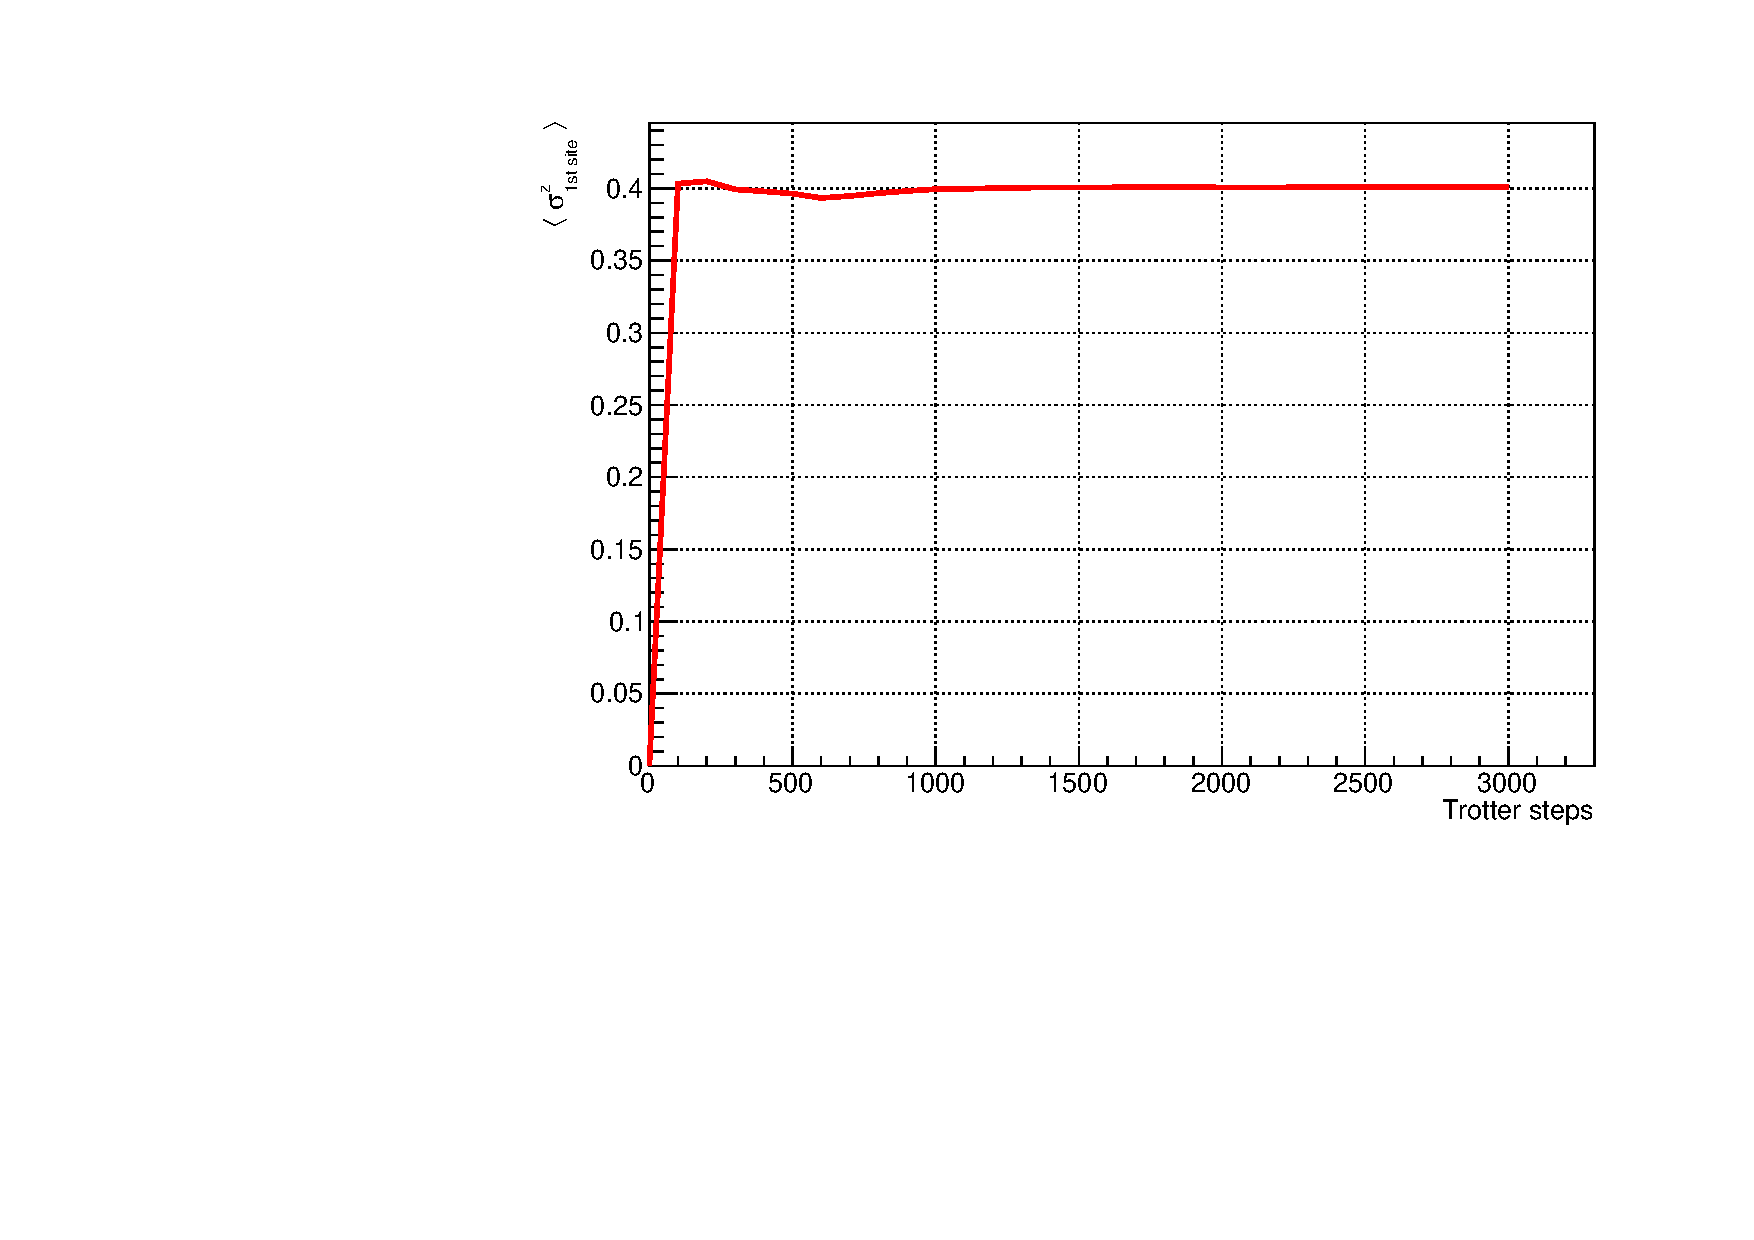
\includegraphics[scale=0.35]{Figures/convergence/Convergence_s8T3000J1051.pdf}
    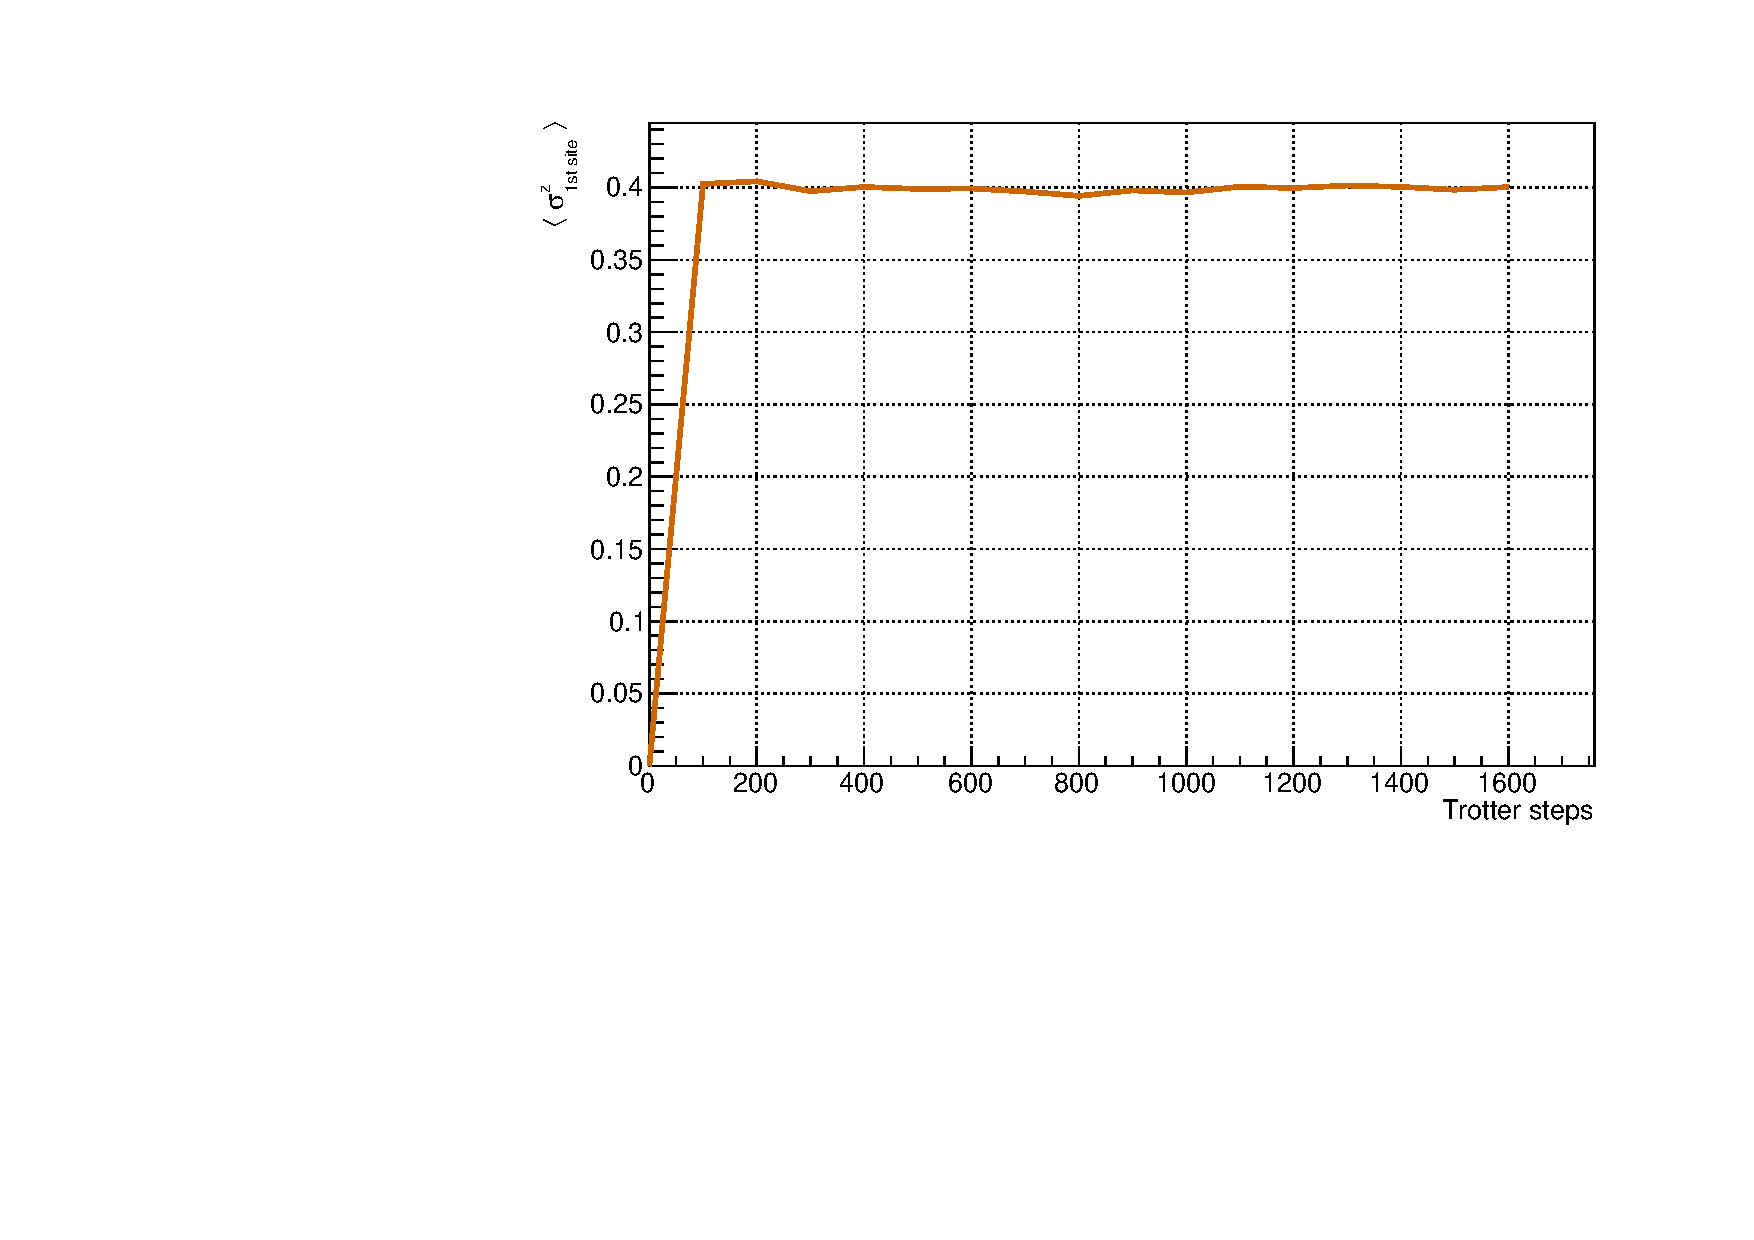
\includegraphics[scale=0.35]{Figures/convergence/Convergence_LM_L012_m060_Time001600_J1051.pdf}
    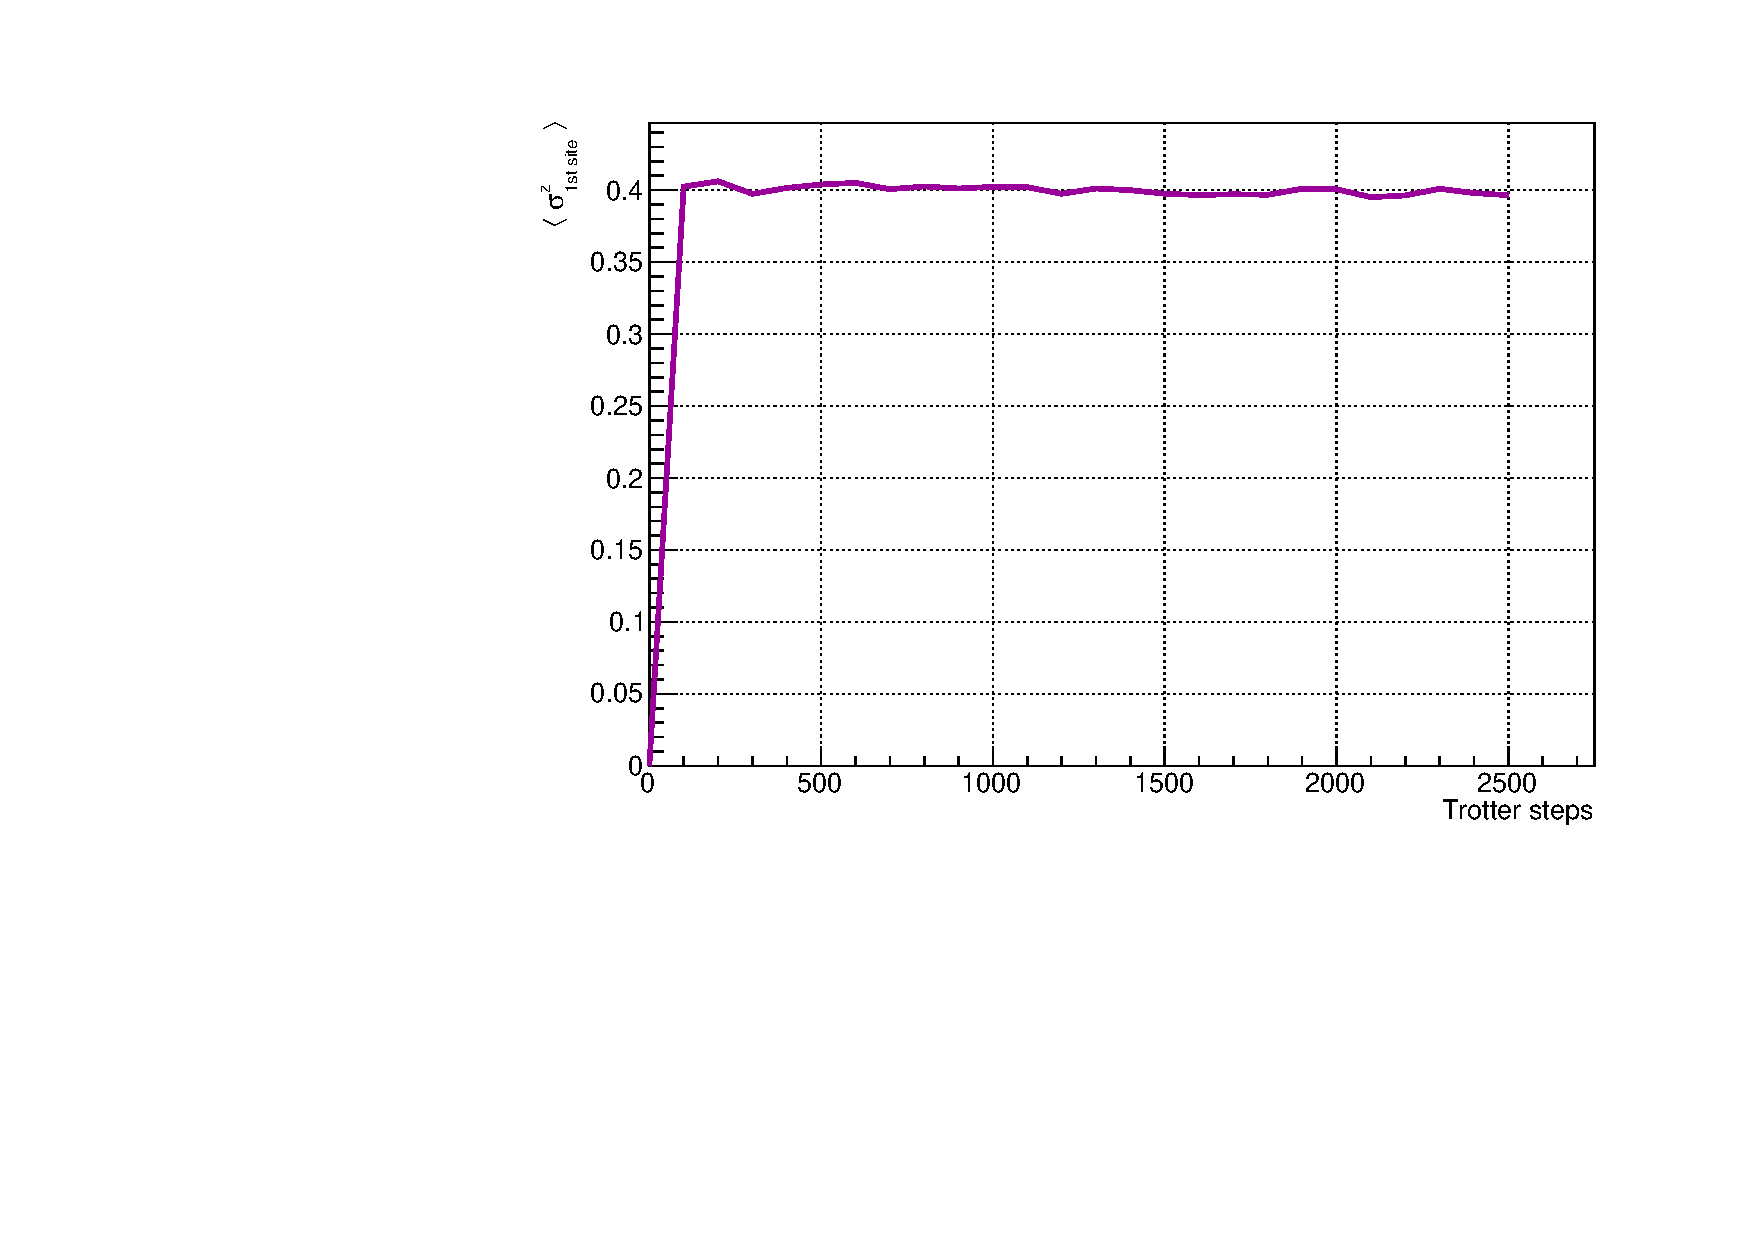
\includegraphics[scale=0.35]{Figures/convergence/ConvergenceLM_L016_m080_Time002500_J1051.pdf}
\captionsetup{width=1.\linewidth}
\caption{Study of convergence of the MPO method for a 8-sites chain, for bond dimension m = 100 and Trotter steps = 3000 (upper-left panel); for a 12-sites chain for bond dimension m = 60 and Trotter steps = 1600 (upper-right panel); for a 16-sites chain for bond dimension m = 100 and Trotter steps = 2500 (bottom panel).}
\label{fig:convergence_8_12_16}
\end{figure}
\\

\pagebreak
\section{Comparison between QT and MPO Results}
As a verification of the plausibility of data obtained from MPO method, we present here a comparison between the data obtained from MPO method and those obtained from QT method, for the analysis of magnetization profile along z direction. In fig.~\ref{fig:LM_comparison_QTvsMPO}, we can see that the results are completely consistent with each other. This is true also for the other observables studied during the thesis work (the two-point correlation function and the spin current) and for other choices of the system parameters (other values of $J_z$ and $\gamma$). Of course the difference of the time needed for reaching the convergence and the ability to reach bigger sizes, makes the MPO method more efficient than QT method.

\begin{figure}[H]
\centering
        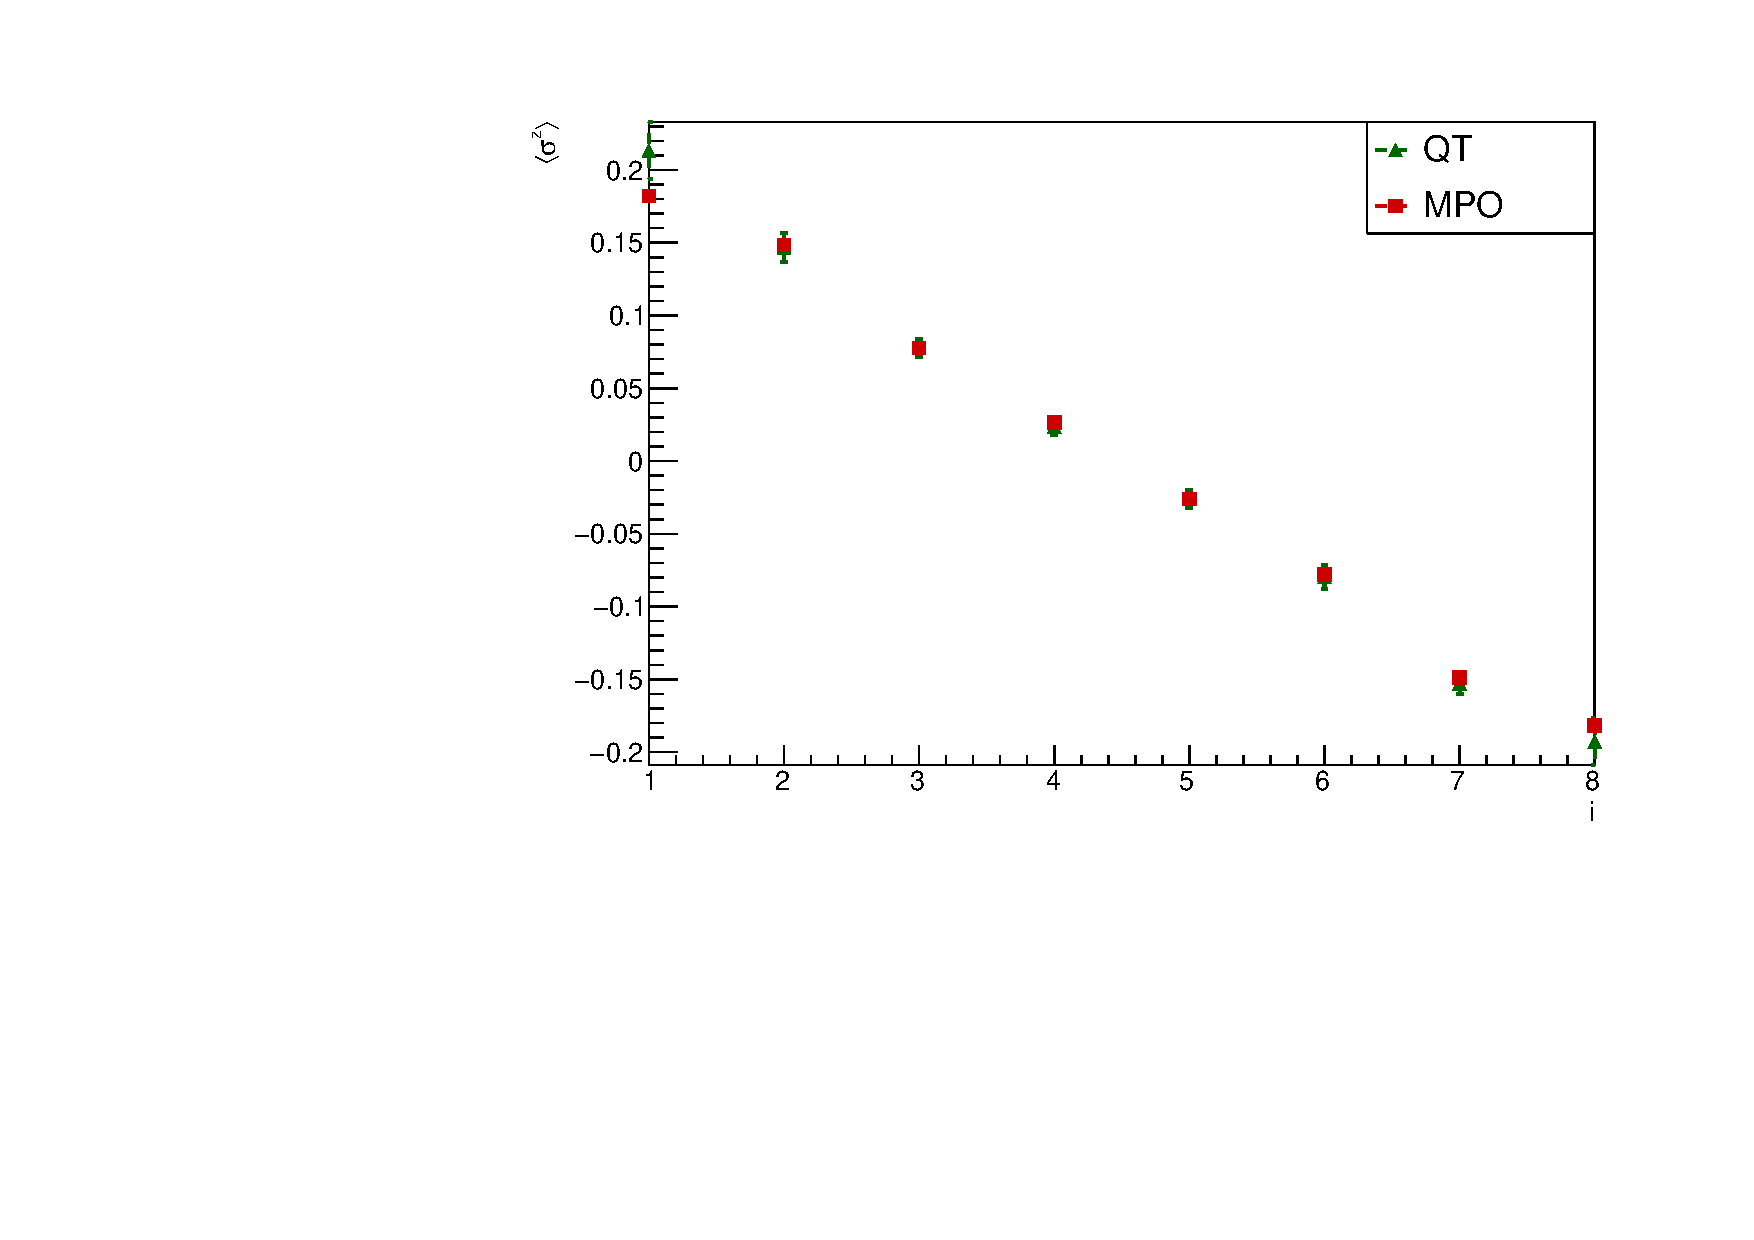
\includegraphics[scale=0.35]{Figures/LMComparison_8sJ10505.pdf}
        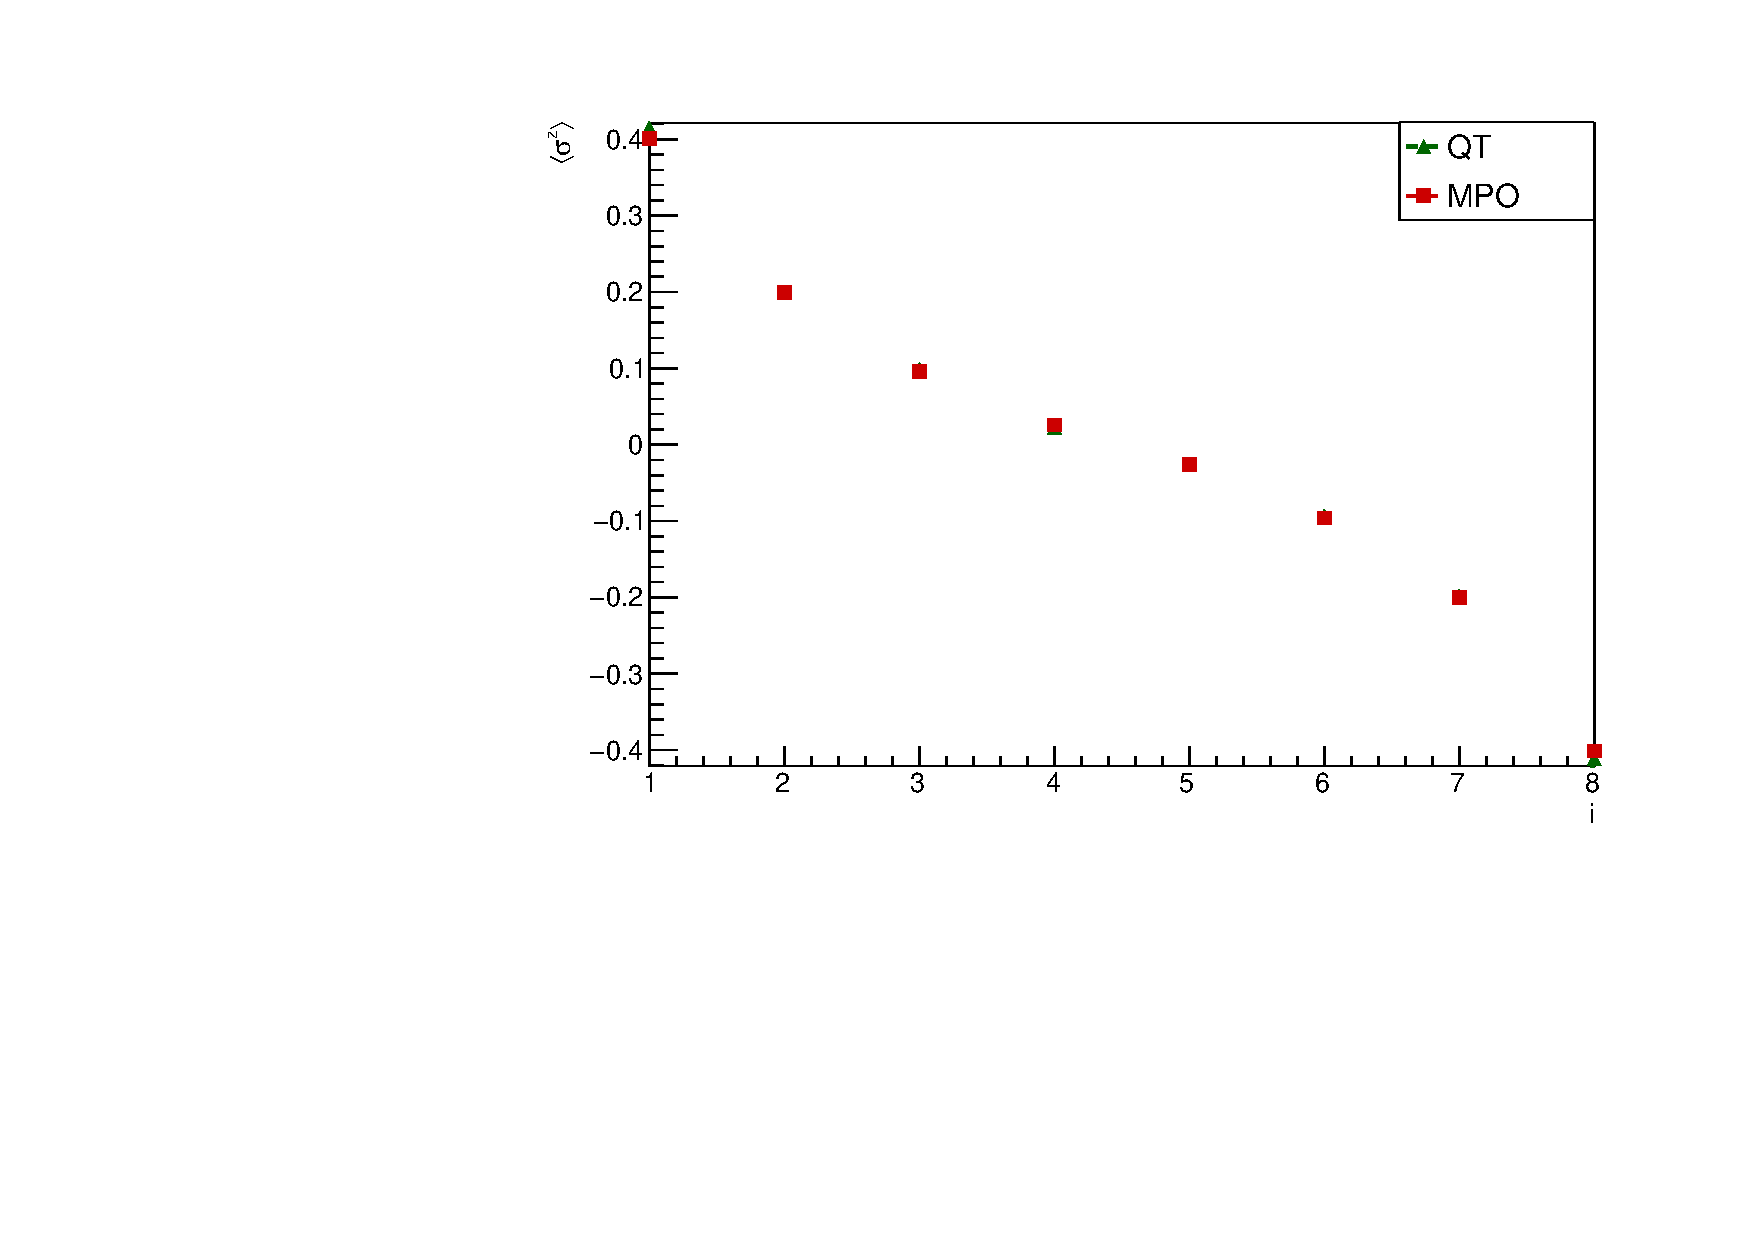
\includegraphics[scale=0.35]{Figures/LMComparison_8sJ1051.pdf}
        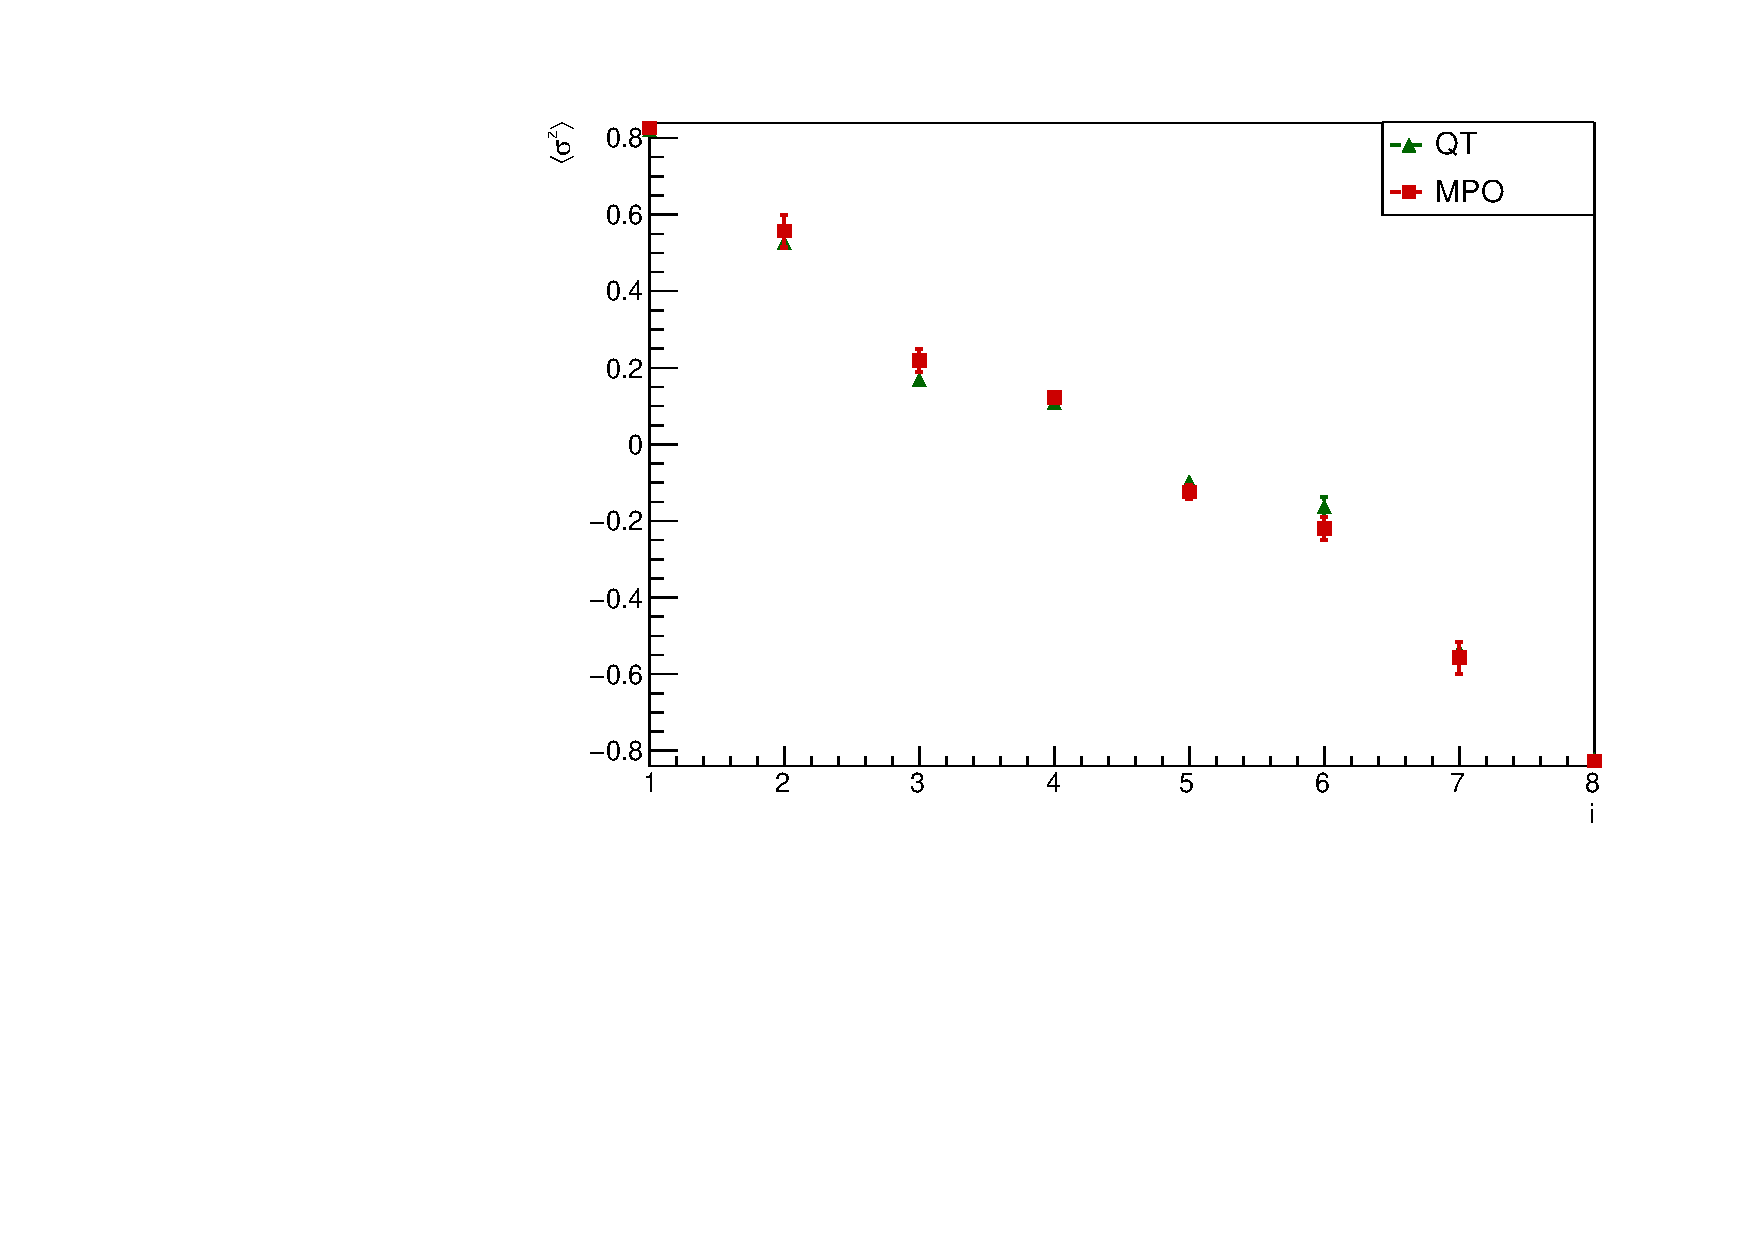
\includegraphics[scale=0.35]{Figures/LMComparison_8sJ10515.pdf}
    \captionsetup{width=1.\linewidth}
    \caption{Magnetization profile for a 8-sites chain for $\gamma = 1$ and $J_z = 0.5$ (upper-left panel), $J_z = 1$ (upper-right panel), $J_z = 1.5$ (bottom panel). Data are obtained from MPO method (in red) and QT method (in green). The error bars are obtained as explained in the above sections.}
    \label{fig:LM_comparison_QTvsMPO}
\end{figure}